\documentclass [11pt, a4paper] {article}

\title{Object State Diagram in Secondo System}

\author{Victor Teixeira de Almeida }

\date{\today}

\usepackage[dvips]{graphicx}
\usepackage[all]{xy}

\begin{document}

\maketitle

\input{macros.tex}

\section{Introduction}
\label{sec:intro}

This document is intended as a documentation of the state diagram of objects inside the Secondo system. This state diagram is needed because objects can have some persistent part handled by its own algebra. Every object in the Secondo system must have a memory part and may have a persistent part not handled by the Secondo system, but by the algebra from which the object belongs. 

In this way, objects, when they exist in the Secondo system, can stay into two states: \emph{opened} and \emph{closed}. The figure \ref{fig:objstatediag} shows the state diagram for objects in the Secondo system. When an object is in \emph{opened} state, it has the memory part already loaded into memory and the files/records needed for the persistent part (if used) are opened and ready for use. When an object is in \emph{closed} state the files/records needed for the persistent part are closed and the memory part is freed. 

\begin{figure}[!hbp]
  \begin{center}
  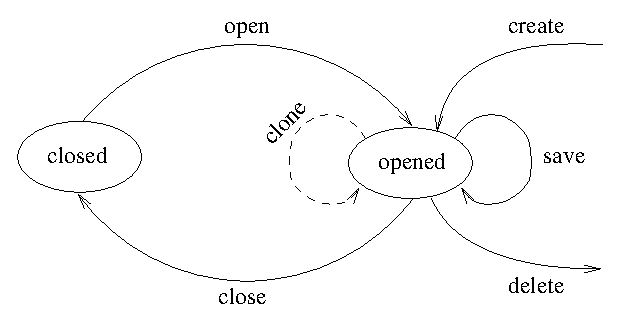
\includegraphics{objstatediag.eps}
  \end{center}
  \caption{Object state diagram.}
  \label{fig:objstatediag}
\end{figure}

Every type constructor must implement these six transition functions, namely \emph{create}, \emph{delete}, \emph{open}, \emph{close}, \emph{save}, and \emph{clone}. The \emph{create} transition creates an object in the system and allocates memory for its memory part and creates files/records (if needed) for its persistent part, in summary, it looks like a constructor of the object. The \emph{delete} transition is the contrary of the \emph{create} one, it takes an opened object and deletes both memory and persistent parts. Like the \emph{create} transition, the \emph{delete} one looks like the destruction of the object. The \emph{close} transition takes an opened object and closes it without deleting it, i.e., deletes the memory part and closes the persistent part. The \emph{open} transition puts again an object into the \emph{opened} state allocating the memory part of the object and reading the persistent part from file/records. The \emph{save} transition is applied to an opened object and does not change the state of the object, but only saves the persistent part of it. Finally, the \emph{clone} transition also takes an opened object and does not change it. This transition returns a newly created object (in opened state) which is a copy of the first one.  
     
How the main commands for objects (\emph{create}, \emph{update}, \emph{delete}, and \emph{query}) use these transition functions will be presented in the next sections.

\subsection{Create command}

Creation of objects in the Secondo system only store necessary information in the catalog and do not really call the create function for storing space for the object in the system. The objects are created with the \emph{defined} flag set to \emph{false}, so the query processor knows that they were not initialized.

\subsection{Delete command}

This command deletes an object previously stored in the Secondo system. It needs then to call the \emph{delete} transition function, but once all objects are in \emph{closed} state, this command needs to open it first. If the object is not defined then this command do nothing. The example below shows the sequence of transition function calls for the delete command.

\begin{table}[h]
\begin{pseudocode}
delete x \\
\\
if( defined ) \\
\{ \\
\> open( x ); \\
\> delete( x ); \\
\}
\end{pseudocode}
\end{table}

\subsection{Update command}

The update command must be divided into three categories. The first one is when an object is being updated with a value calculated by the query processor. This value can be the result of a math computation, for example, or the application of an operator, or even a series of operators. The example below shows the sequence of transition function calls for the this first kind of update command. In this kind of update command, the object $x$ needs first to be deleted if it is defined. Then a new object is created by the query processor, the 0 is done, and the object $x$ is saved and closed. The opening and closing of the objects ($y$) used in the right side of the 0 will be done by the query processor and will be explained in the \emph{query} command.

\begin{table}[h]
\begin{pseudocode}
update x := [y] \\
\\
if( defined ) \\
\{ \\
\> open( x ); \\
\> delete( x ); \\
\} \\
save( x ); \\
close( x ); \\
\end{pseudocode}
\end{table}

The second type of an update command is when a real update of an object occur. The object, in this kind of update, is not being assigned a value, but updating itself. The example below shows the sequence of transition function calls for the this second kind of update command. This command can be the resulting of an operation like $inc(x)$, for example, which takes an integer value $x$ and increments its value by $1$. In this kind of operation, it is just needed to save the new value of the object $x$ and close it. The object $x$ must be necessarily created before this command.

\begin{table}[h]
\begin{pseudocode}
x := [x] \\
\\
save( x ); \\
close( x ); \\
\end{pseudocode}
\end{table}

The third and the last kind of update command is when an object is assigned directly a value of another object. The example below shows the sequence of transition function calls for the this third kind of update command. This case need to be handled differently because a clone of the object $y$ in the right side of the 0 must be done before the real 0. This command begins like the first one deleting (if necessary) the object $x$. Then, the object $y$ is opened, cloned, and assigned to the object $x$. The object $x$ is then saved and both are closed.  

\begin{table}[h]
\begin{pseudocode}
x := y \\
\\
if( defined ) \\
\{ \\
\> open( x ); \\
\> delete( x ); \\
\} \\
open( y );  \\
x = clone( y ); \\
save( x ); \\
close( x ); \\
close( y ); \\
\end{pseudocode}
\end{table}

\subsection{Query}

In queries, the object creation, deletion, opening, and closing will be done by the query processor. The query processor constructs a query tree which looks like the one in figure \ref{fig:querytree}. The circles represent internal nodes of the tree where the objects need to be created and then deleted to receive the result of operations. The rectangles represent leaf nodes of the tree where there can exist objects and constants. If the leaf node contains an object, the objece needs only to be opened and closed. If it contains a constant, the constant needs to be created and deleted. 

\begin{figure}[!hbp]
  \begin{center}
  \includegraphics{querytree.eps}
  \end{center}
  \caption{Object manipulation in the query tree.}
  \label{fig:querytree}
\end{figure}

\end{document}
